\chapter{Introduction}
	Today there are over 3.5 million km of transmission pipelines in the world. 231~900 km pipelines
	are planned or under construction \cite{DNV_pipelines}. Pipelines currently in place need to
	continue operating, many of them far longer than they were initially intended. Great effort are taken
	to inspect and maintain the pipelines to keep them in satisfying order.  The pipeline needs to be 
	in working order to be operational.
	Potential leaks might cause irreversible environmental damages, and companies looses money when the
	flow through the pipeline are stopped. 

	There are two ways of inspecting pipelines; \textit{internal} and \textit{external} 
	inspection. The internal inspection methods, includes stopping the flow in the pipeline,
	open it and insert a Pipeline Inspection Gauge (PIG) which travels inside the pipeline and uses various
	sensors to determine the state of the pipeline. The other method, \textit{exterior} pipeline
	inspections are today mostly done using Remotely Operated Vehicles, ROVs. The ROVs are tethered
	unmanned underwater vehicles, and are the work horse of the offshore industry. They are versatile
	tools capable of accomplishing most missions associated with pipeline inspections and repair. However,
	they need well-equipped, expensive support vessels and a large crew to accompany the inspection
	mission which of course are very costly for the pipeline owner. British Petroleum stats that the ROV
	are ``overactuated'' for the pipeline inspection case.\cite{pipelines}

	An Autonomous Underwater Vehicle (AUV) is a suiting tool for pipeline inspection. An AUV is a
	untethered unmanned underwater vehicle. Opposed to the ROVs, which operation radius are limited by the
	tether, the operation radius of the AUV are limited by power consumption and battery life. 
	An AUV comes in many forms, small or large. It may need minimal support crew which will minimise the
	cost for the pipeline owners. It can be made small enough to be launched from small ships, and even
	from shore to inspect pipelines going to the oil refinery on land. This would be a great advantage
	for the pipeline owners to cut costs, instead of hiring large support vessels and crew to support a
	pipeline inspection mission.
	
	The speed of the inspections is also an important issue. A typical ROV has cruise speeds from $1-2$
	knots ($0.5-1$ m/s), while an AUV has cruise speeds in the regime $2-6$ knots ($1-3$ m/s). This
	inclines that an AUV might cover larger area of pipelines than an ROV. 

	British Petroleum estimates that they can save up to 30 \% by using AUVs for pipeline inspections
	instead of ROVs, which motivates the research in the area. The market for AUV doing pipeline
	inspections are present. The technology needed are present, and there are a number of companies developing
	AUVs for pipeline following. SeaByte and Subsea7 have conducted a successfull pipeline inspection
	mission using the \textit{Geosub} AUV and claimed the world record in the longest uninterrupted
	pipeline inspection mission. The AUV inspected 22.2 km of pipeline at $4$ knots without being
	interrupted. \cite{Seabyte}, \cite{PhD_lecture}
	
	This report will look at the possibility to give the Kongsberg Maritime \hugin AUV the
	given abilities to track and follow a subsea pipeline. The AUV have hovering capabilities and are
	controllable in 5 degrees of freedom (DOF).The AUV are assumed stable in the \textit{roll}.
	Although, the hovering abilities are present, this will not be used when designing the guidance
	system, because of the focus on energy efficiency.

	\begin{figure*}[htbp]
		\centering
		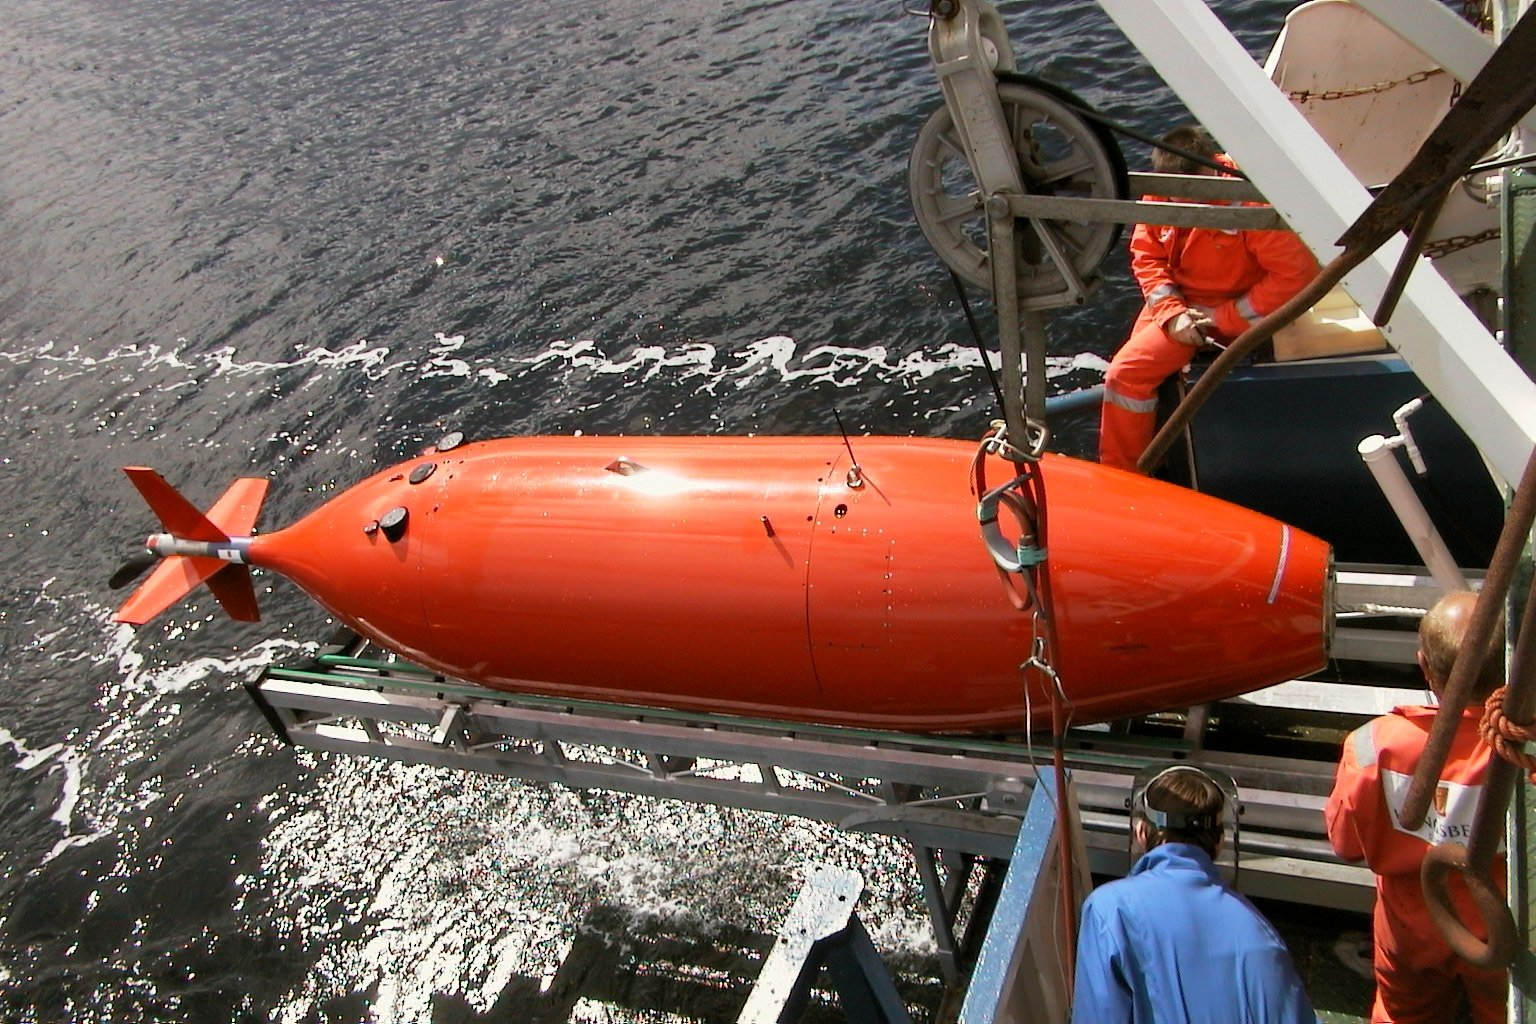
\includegraphics[width=0.8\textwidth]{pics/hugin3000}
		\caption[\textit{HUGIN} Vehicle]{\textit{HUGIN 3000} under launch. \hugin are somewhat 
		smaller than \textit{HUGIN 3000} but identical in shape. \textit{xpda.com}}
	\end{figure*}

	The pipeline detection equipment is a downward looking camera with sufficient lighting to operate at about
	3-5 meters above the seabottom. Of course the visibility conditions will change according to depth and
	amount of particles in the water. This is probably an optimistic assumption, and at great
	depth the visibility will probably be less than 3 meters.

	This report considers how to automate the pipeline inspections process. It will consider the
	possibility that the pipeline is buried under mud and not visible to the camera or buried on purpose
	to make it more robust towards environment forces and erosion, in both cases the important thing 
	is to reacquire the pipeline at the end of the buried stretch. In that case some kind of an
	estimator have to be used to predict where the pipeline is headed.
	
	A pipeline inspection mission can be divided into 4 parts:
	\begin{enumerate}
	 \item Initialisation and initial descent
	 \item Search for and Acquire pipeline
	 \item Track and Inspect pipeline
	 \item Ascent to the surface and deliver the acquired data
	\end{enumerate}

	The \textit{Initial descent} and \textit{final ascent} are self explanatory. But what happens if the
	pipeline are not at the initial position when, when the AUV arrives at that location? It is obvious
	that some kind of search need to be initiated. 
	
	The \textit{Search and Acquire} part will need the vessel to move in some kind of search pattern if
	the pipeline is not located exactly where the initial position data states it to be. This search
	pattern should also be used if the pipeline is lost during tracking. 
	
	The \textit{Track and Inspect} part needs a guidance system which is capable of keeping the vessel 
	on top of the pipeline or in the vicinity, independent of the current in the area and other possible 
	disturbances. This is
	necessary because the primary mission for the AUV is to provide video of the pipeline which can be
	used to determine the state and well-being of the pipeline.
	
	This report is divided into four chapters;
	\begin{enumerate}
	 \item Theory. Describes the necessary theory needed to understand the proposed guidance system, and
	contains a summary of literature on the pipeline following subject.
	 \item Modeling, assumptions about the model and how it is modeled. A Kalman Filter and a flight-mode
	 controller will be derived. A guidance system will be proposed and desired behaviour will be
	 addressed.
	 \item Implementation and simulation of the proposed system. How the system is implemented and how it
	 performs in certain situations will be treated in this chapter. 
	 \item Discussion of the results given by the simulations, and various aspects about the proposed
	 guidance system will be discussed. A review of how valid the results will also be given here.
	 \item Summary of the results, together with conclusion and future work will be treated in the last
	section.
	\end{enumerate}

	
	
	

